\documentclass[a4paper, 11pt]{article}
\usepackage{comment} % enables the use of multi-line comments (\ifx \fi) 
\usepackage{fullpage} % changes the margin
\usepackage{pdflscape}
\usepackage{rotating}
\usepackage{graphicx}
\usepackage[table]{xcolor}

\begin{document}
%Header-Make sure you update this information!!!!
\noindent
\large\textbf{Program Assignment 2} \hfill \textbf{Longxiang Li} \\
\normalsize CS124 \hfill Teammates: No \\

\section*{Introduction}
Strassen's matrix multiplication algorithms works faster for $n$ by $n$ matrix than the conventional naive algorithm whose time complexity is $O(n^3)$, in theory. However, for some smaller n, the conventional algorithm runs faster because the time consumed in memory allocation in Strassen's algorithm. But, for this recursive algorithm, we don't need to go to the basic element of this matrix (a $1\times1$). We may modified the classic algorithm by converting from recursion to conventional algorithm when the dimension is small enough. We call this cross-over point. In this experiment, we try to find the optimal cross-over point for different $n$ from two direction. First, we calculate the exact running time for Strassen's algorithm, modified Strassen's algorithm and conventional algorithm and estimate the cross-over point numerically. These calculation were based on the assumption that the cost of any single arithmetic operation is 1 and all others are free. Second, we implemented these algorithms and get the cross-over point in practice.
\section*{Numerical Calculation}
To simplify the calculation we assume in the following analysis in this section, the dimension n is power of 2 and the cross-over value is also power of 2. In classic Strassen's algorithm, for a given matrix of given $n$, we require 7 multiplication of matrices of simension $\frac{n}{2}$. In addition, there are 18 summation and subtraction of size $\frac{n}{2}$. Thus, we can write a recursive equation of the running time:
\[{f_1}(n)=7f(\frac{n}{2})+18(\frac{n}{2})^2\] 
\[=7^2f(\frac{n}{4})+7\times18 (\frac{n}{4})^2+18(\frac{n}{2})^2\] 
\[=7^kf(\frac{n}{2^k})+18n^2\{7^{k-1}(\frac{n}{2^k})^2+\dots+7^0(\frac{n}{2})^2\}\]
when $k=log_2{n}$, we arrive at the basic case. Since $f(1)=1$. We can conclude that the exact running time of standard Strassen's algorithm is:
\[f_s(n)=7^{log_2{n}}+6n^2\{(\frac{7}{4})^{log_2{n}}-1\}\]
For conventional algorithm, we have a total of $n^3$ multiplication and $n^2(n-1)$ additions. So the close form running time of conventional algorithm is:
\[f_c(n)=n^2(2n-1)\]
Let's assume we set cross-over point at $n_0$. That means above $n_0$, we used Strassen's algorithm and below $n_0$, we used conventional algorithm. So the running time of this hybrid algorithm is:
\[f_{n_0}=7^{log_2{\frac{n}{n_0}}}(2n_0^3-n_0^2)+6n^2((\frac{7}{4})^{log_2{\frac{n}{n_0}}}-1)\]

We cannot achieve a closed form $n_0$ for every $n$. But we can get a numeric estimation. The theoretical running time of standard Strassen's, modified Strassen's with $2\times2$, $4\times4$, $8 \times 8$, $16 \times 16$ basic matrix and conventional algorithm are listed below:
\begin{table}[ht]
	\centering
	\caption{theoretical running time comparison among algorithms up to $2^{12}$}
	\begin{tabular}{rrrrrrrr}
		\hline
		& $n$ & Strassen's & 2*2 & 4*4 & 8*8 & 16*16 & Conventional \\ 
		\hline
		& 16 & 15271 & 10812 & 8656 & 7872 & 7936 & 7936 \\ 
		& 32 & 111505 & 80292 & 65200 &\cellcolor{blue!25} 59712 & 60160 & 64512 \\ 
		& 64 & 798967 & 580476 &\cellcolor{blue!25} 474832 & 436416 & 439552 & 520192 \\ 
		& 128 & 5666497 &\cellcolor{blue!25} 4137060 & 3397552 & 3128640 & 3150592 & 4177920 \\ 
		& 256 & 39960391&  \cellcolor{blue!25}29254332 & 24077776 & 22195392 & 22349056 & 33488896 \\ 
		& 512 & 280902385 &\cellcolor{blue!25} 205959972 & 169724080 & 156547392 & 157623040 & 268173312 \\ 
		& 1024 &\cellcolor{blue!25} 1971035287 & 1446438396 & 1192787152 & 1100550336 & 1108079872 & 2146435072 \\ 
		& 2048 &\cellcolor{blue!25} 13816121377 & 10143943140 & 8368384432 & 7722726720 & 7775433472 & 17175674880 \\ 
		& 4096 &\cellcolor{blue!25} 96788347111 & 71083099452 & 58654188496 & 54134584512 & 54503531776 & 137422176256 \\ 
		\hline
	\end{tabular}
\end{table}
\begin{figure*}[h]
	\centering
	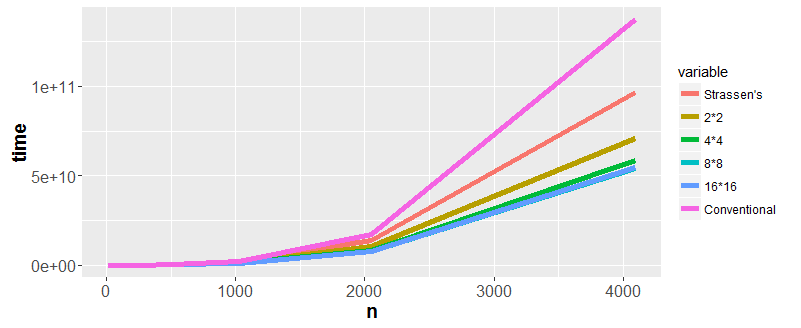
\includegraphics[width=0.7\linewidth]{Numeric}
	\caption[]{theoretical running time comparison among algorithms up to $2^{12}$}
	\label{fig:numericto256}
\end{figure*}
For a matrix with size of $n$, when $n\leq 16$, by no means can Strassen's run faster than conventional algorithm in theory. Then for a matrix of size 32, modified Strassen's with $8\times8$ basic matrix runs faster. In this case, the theoretical cross-over point maybe between 4 and 8. Then for a matrix with 

\section*{Alternative Solutions}

\section*{Optimum Solution}

\section*{Construction/Implementation}

\section*{Analysis \& Testing}

\section*{Final Evaluation}

\section*{Attachments}
\end{document}
